\documentclass[conference]{IEEEtran}
\IEEEoverridecommandlockouts

\usepackage{cite}
\usepackage{amsmath,amssymb,amsfonts}
\usepackage{graphicx}
\usepackage{textcomp}
\usepackage{xcolor}
\usepackage{booktabs}

\graphicspath{{figures/}}

\begin{document}

\title{Paper Title (use style: paper title)}

\author{
\IEEEauthorblockN{First Author}
\IEEEauthorblockA{\textit{Department} \\
\textit{University}\\
City, Country \\
email@example.com}
\and
\IEEEauthorblockN{Second Author}
\IEEEauthorblockA{\textit{Department} \\
\textit{University}\\
City, Country \\
email@example.com}
}

\maketitle

\begin{abstract}
This document is a template for an IEEE conference paper. Replace this text
with your abstract.
\end{abstract}

\begin{IEEEkeywords}
component, formatting, style, insert
\end{IEEEkeywords}

\section{Introduction}
Introduce the problem and cite prior work~\cite{lamport1994}.

\section{Method}
Describe your approach. Equation~\eqref{eq:example} is an example:
\begin{equation}
  a + b = \gamma \label{eq:example}
\end{equation}

\section{Results}
\begin{figure}[htbp]
  \centering
  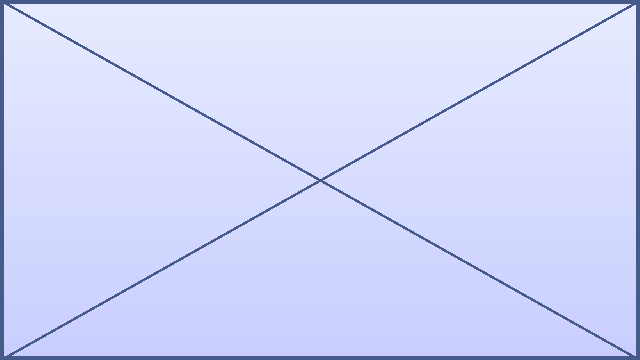
\includegraphics[width=\columnwidth]{placeholder.png}
  \caption{Example figure.}
  \label{fig:example}
\end{figure}

\begin{table}[htbp]
  \caption{Example table}
  \centering
  \begin{tabular}{lcc}
    \toprule
    Method & Metric A & Metric B \\
    \midrule
    Baseline & 0.71 & 0.65 \\
    Ours & \textbf{0.84} & \textbf{0.79} \\
    \bottomrule
  \end{tabular}
  \label{tab:example}
\end{table}

\section{Conclusion}
Summarise your findings.

\bibliographystyle{IEEEtran}
\bibliography{references}

\end{document}
